\documentclass{ctexbeamer}
\usepackage{minted}
\usepackage{graphicx}
\usepackage{amssymb, amsmath, amsfonts}

\usefonttheme{serif}
\usetheme{CambridgeUS}

\setlength{\parskip}{0.5em}

\setminted{
    % fontsize=\small,           % 字体大小
    baselinestretch=1.0,       % 行间距
    % linenos=true,              % 行号
    frame=single,           % 边框样式
    framesep=2mm,              % 边框间距
    rulecolor=\color{black},   % 边框颜色
    % numbersep=5pt,             % 行号间距
    breaklines=true,           % 自动换行
    breakanywhere=false,       % 不在任意位置断行
    showspaces=false,          % 不显示空格
    showtabs=false,            % 不显示制表符
    tabsize=4,                 % 制表符大小
    % url=false,
}

\title{第三次上机课}
\author{臧炫懿}
\date{\today}

\begin{document}

\frame{\titlepage}

\begin{frame}
    \frametitle{目录}

    \tableofcontents

\end{frame}

\section{机器学习与PyTorch的使用}

\frame{\sectionpage}

\subsection{数学基础}

\begin{frame}
    \frametitle{机器学习干了个什么事？}

    其实正课最让人诟病的一点就是这个，它没有讲清楚机器学习\textbf{到底在做什么}。

    \hspace{1em}
    \begin{center}
        \Large \textbf{机器学习是一个从数据中学习模型来进行预测的过程。}
    \end{center}

    于是从这个定义出发，我们有着不同的范式：监督学习、无监督学习、自监督学习、强化学习等，其难度大致递增。我们上课首先讲的是线性回归，但线性回归甚至不是最简单、也不是最好理解的SL。

    最简单的SL实际上是\textbf{分类}问题。本节课我将以分类问题为例来讲解机器学习的数学基础。

\end{frame}

\begin{frame}
    \frametitle{入门级别的分类问题：MNIST-10数据集分类}

    MNIST-10数据集分类问题是最经典的入门级别的分类问题。

    考虑以下问题：现在有一百万张图片（$28\times 28 \times 1$），每张图片上都有一个数字（0-9），现在我们想要训练一个模型，输入一张图片，输出图片上的数字。

    乍一看，这个问题似乎是很难的，让我们无从下手。

\end{frame}

\begin{frame}
    \frametitle{简化问题}

    现在平面上有一堆点，每个点都有一个标签（0或1），现在我们想要训练一个模型，输入一个点的坐标，预测这个点的标签。

    \hspace{2em}
    \pause

    显然，如果\textbf{划一条合适的线}，就能把这两个类别分开了。

    实际上这就是机器学习分类问题的核心：\textbf{划线}。

\end{frame}

\begin{frame}
    \frametitle{怎么划线？}

    于是划线：
    \[ \mathbf{W}^\top \mathbf{x} + b = 0 \]

    得到函数$f(\mathbf{x}) = \mathbf{W}^\top \mathbf{x} + b$，如果$f(\mathbf{x}) > 0$，就预测标签为1；如果$f(\mathbf{x}) < 0$，就预测标签为0。

    人类是可以看着图找到这条线的。但是如果要把这个东西形式化成一个计算机可以做的算法，那仅凭人类的经验是不可以的。

    算法两要素：\textbf{形式化}、\textbf{有限终止}。好的算法必须满足这两点，实在不行可以放弃有限终止，但绝对不可以放弃形式化。

    既然这样，问题就变成了：
\begin{center}
    \Large\color{blue} \textbf{如何形式化地划一条线？}
\end{center}

\end{frame}

\begin{frame}
    \frametitle{损失函数}

    那下一个问题就变成了

    \begin{center}
        \Large\color{blue}  \textbf{怎样形式化地定义线的好坏？}
    \end{center}

    利用函数思想，我们一般把线的好坏用一个\textbf{损失函数}来衡量。因为一般“好”是无上限的，但“坏”是有下限的，所以我们一般把损失函数定义为一个非负的函数，且当预测结果和真实标签完全一致时，损失函数的值为0；当预测结果和真实标签完全不一致时，损失函数的值较大。

    于是显然有一个比较初级的损失函数：
    \[ \mathcal{L} = \sum \mathbb{I} \{ \hat{y} \neq y \} \]

    现在可以使用搜索来解决问题。

\end{frame}

\begin{frame}
    \frametitle{传统搜索的局限性}

    但是传统搜索的局限性也很明显。\textbf{你总不能在$\mathbb{R}^n$里进行搜索吧？}

    那为什么不能直接求解方程$\mathcal{L} = 0$呢？

    因为这个方程的解可能并不存在——谁说数据一定是完美的、可以被划线分开的了？就算我们取的数据是个好的数据，但也会有噪声、异常值等问题，这些都会导致这个方程的解不存在了。

    我们必须要换个方法来找到这个损失函数的最小值。

\end{frame}

\begin{frame}
    \frametitle{导数等于零！}

    数学告诉我们，如果一个函数光滑，那么我们就可以通过求导数，并使得其导函数的值为0来找到这个函数的极值点。于是我们就可以利用这个方法来获得损失函数的最小值。

    于是定义一个新的损失函数：
    \[ \mathcal{L} = \sum (\hat{y} - y)^2 \]
    这个损失函数的值就是预测结果和真实标签之间的平方误差。这个损失函数是一个光滑的函数，我们就可以通过求导数来找到它的最小值：
    \[\frac{\partial \mathcal{L}}{\partial \mathbf{W}} = 0, \quad \frac{\partial \mathcal{L}}{\partial b} = 0\]

    但问题又来了：\textbf{这个方程的解可能也不存在——至少解析解求起来会非常艰难！}

\end{frame}

\begin{frame}
    \frametitle{导数等于零？}

    那二分法呢？其实问题还是一样的：在$\mathbb{R}^n$里进行二分也是极为不现实的。

    于是我们继续被迫寄希望于数学家——这时，我们找到了牛顿：
    \[x_{n+1} = x_n - \frac{f(x_n)}{f'(x_n)}\]
    牛顿法求方程$f(x) = 0$的数值解，形式化，可操作！

    当然我们这里求的是$f'(x) = 0$的数值解了，那么我们就可以把上式中的$f(x)$换成$f'(x)$，得到：
    \[x_{n+1} = x_n - \frac{f'(x_n)}{f''(x_n)}\]

\end{frame}

\begin{frame}
    \frametitle{牛顿优化法面临的问题和梯度下降法的由来}

    于是，我们现在试图把原来的这个$\mathcal{L}$带进上式：
    \[(\mathbf{W}_{n+1}, b_{n+1}) = (\mathbf{W}_n, b_n) - \frac{\nabla \mathcal{L}(\mathbf{W}_n, b_n)}{\nabla^2 \mathcal{L}(\mathbf{W}_n, b_n)}\]
    这就是大名鼎鼎的\textbf{牛顿优化法}。

    实际上，牛顿优化法在实际应用中面临的最大问题是这个$\mathbf{W}$可能是一个非常高维的向量（甚至是一个矩阵），而且$\nabla^2 \mathcal{L}$要求逆，这就导致了计算复杂度非常高（$O(n^3)$），在实际应用中是不可行的。

    二阶优化大失败！（当然二阶优化因为收敛快，在某些特定的场景下还是有用的，例如BFGS算法）

\end{frame}

\begin{frame}
    \frametitle{一阶优化：梯度下降法}
    \[(\mathbf{W}_{n+1}, b_{n+1}) = (\mathbf{W}_n, b_n) - \frac{\nabla \mathcal{L}(\mathbf{W}_n, b_n)}{\nabla^2 \mathcal{L}(\mathbf{W}_n, b_n)}\]

    再次观察上式，发现这个Hessian矩阵的逆其实是用来调整梯度的步长的，那么我们就可以把它近似成一个常数，这样就得到了\textbf{梯度下降法}：
    \[(\mathbf{W}_{n+1}, b_{n+1}) = (\mathbf{W}_n, b_n) - \eta \nabla \mathcal{L}(\mathbf{W}_n, b_n)\]

    这里的$\eta$就是\textbf{学习率}，替代牛顿优化法中的Hessian矩阵的逆（也就是二阶导数），使得算法的计算复杂度从$O(n^3)$降低到了$O(n)$，在实际应用中可行。

\end{frame}

\begin{frame}
    \frametitle{链式法则}

    尽管我们得到了一个可以用来迭代$\mathbf{W}$和$b$的算法，但是……

    \textbf{你怎么去对一个矩阵求偏导数？}

    实际上对矩阵求导确实有严格定义，但是非常麻烦，会搞出来一些逆变或协变的东西。机器学习本质上也不需要那么严谨，其实我们可以暂时形式化地认为以下链式法则是成立的（至少结果基本上是对的）：
    \[\frac{\partial \mathcal{L}}{\partial \mathbf{W}} = \frac{\partial \mathcal{L}}{\partial \hat{y}} \cdot \frac{\partial \hat{y}}{\partial f} \cdot \frac{\partial f}{\partial \mathbf{W}}\]
    \[\frac{\partial \mathcal{L}}{\partial b} = \frac{\partial \mathcal{L}}{\partial \hat{y}} \cdot \frac{\partial \hat{y}}{\partial f} \cdot \frac{\partial f}{\partial b}\]
    可能学数学的同学看到这一步会生气，但我们先不去管它。
\end{frame}

\begin{frame}
    \frametitle{实例练习}

    假设损失函数$\mathcal{L} = (\hat{y} - y)^2$，神经网络为单层二维线性分类器$f(\mathbf{x}) = \mathbf{W}^\top \mathbf{x} + b$叠加一个sigmoid输出层$\hat{y} = \sigma(f(\mathbf{x}))$，其中$\sigma(z) = 1/(1 + e^{-z})$。

    具体数值：$\mathbf{x}_\text{in} = [2, 3]^\top$，$y = 1$，$\mathbf{W} = [1, 2]^\top$，$b = 3$。学习率$\eta = 0.1$。

    试着求出：$\mathbf{x}_\text{out}$、$\hat{y}$、$\mathcal{L}$、经过一次迭代后的$\mathbf{W}$和$b$的值。本题目仅用于说明问题，数据比较极端，仅用纸笔计算近乎不可能得到答案，所以列出算式即可。

    \hspace{2em}

    \pause

    先进行前向传播：
    \[f(\mathbf{x}_\text{in}) = \mathbf{W}^\top \mathbf{x}_\text{in} + b = [1, 2] \times [2, 3]^\top + 3 = 1 \cdot 2 + 2 \cdot 3 + 3 = 11\]
    \[\hat{y} = \sigma(f(\mathbf{x}_\text{in})) = \sigma(11) \approx 0.999983\]
\end{frame}

\begin{frame}
    \frametitle{实例练习的解答：求导数部分}

    \[\frac{\partial \mathcal{L}}{\partial \hat{y}} = 2(\hat{y} - y) = 2(0.999983 - 1) = -0.000034\]
    \[\frac{\partial \hat{y}}{\partial f} = \sigma'(f) = \sigma(f)(1 - \sigma(f)) = 0.999983 \cdot (1 - 0.999983) = 0.000017\]
    \[\frac{\partial f}{\partial \mathbf{W}} = \mathbf{x}_\text{in} = [2, 3]^\top\]
    \[\frac{\partial f}{\partial b} = 1\]

    这个练习中，叠加一个Sigmoid输出层的主要原因是：将输出数值保序地映射到0和1之间——因为这个题目只有0或1两类标签，若是预测值在0和1以外，反而不好解释。

\end{frame}

\begin{frame}
    \frametitle{实例练习的解答：梯度计算和反向传播}

    \[\frac{\partial \mathcal{L}}{\partial \mathbf{W}} = \frac{\partial \mathcal{L}}{\partial \hat{y}} \cdot \frac{\partial \hat{y}}{\partial f} \cdot \frac{\partial f}{\partial \mathbf{W}} = [-0.000001156, -0.000001734]^\top\]
    \[\frac{\partial \mathcal{L}}{\partial b} = \frac{\partial \mathcal{L}}{\partial \hat{y}} \cdot \frac{\partial \hat{y}}{\partial f} \cdot \frac{\partial f}{\partial b} = -0.000034 \cdot 0.000017 \cdot 1 = -0.000000578\]
    \[\mathbf{W}_\text{new} = \mathbf{W} - \eta \cdot \frac{\partial \mathcal{L}}{\partial \mathbf{W}}  = [1.0000001156, 2.0000001734]^\top\]
    \[b_\text{new} = b - \eta \cdot \frac{\partial \mathcal{L}}{\partial b} = 3 - 0.1 \cdot (-0.000000578) = 3.0000000578\]

\end{frame}

\begin{frame}
    \frametitle{形式化的训练过程}

    有了这个，我们就发现了一个非常好的算法了：
    \begin{enumerate}
        \item 随机划线$\mathbf{W}^\top_0 \mathbf{x} + b_0 = 0$，再叠加合适的输出层，得到预测结果$\hat{y}_0$。
        \item 计算对应的损失函数的值$\mathcal{L}_0$。
        \item 根据损失函数的值来调整$\mathbf{W}$和$b$，得到新的划线$\mathbf{W}^\top_1 \mathbf{x} + b_1 = 0$，得到新的预测结果$\hat{y}_1$。
        \item 重复上述过程，直到损失函数的值足够小了。
        \item 用这个划好的线来预测新的数据。
    \end{enumerate}

\end{frame}

\begin{frame}
    \frametitle{前向传播、反向传播等}

    刚刚这个算法包括以下几个部分：
    \begin{itemize}
        \item 前向传播：从输入到预测值的过程。
        \item 反向传播：从预测值、损失函数的值去更新参数的过程。
        \item 训练过程：循环进行前向传播和反向传播的过程。
        \item 预测过程：用训练好的模型来预测新的数据的过程，这时仅进行前向传播，不进行反向传播了。
    \end{itemize}

    实际上这就是机器学习的核心过程！

\end{frame}

\begin{frame}
    \frametitle{从划线到划超平面}

    于是我们试图来解释下一个问题（比原问题简单）：

    现在要试图辨认一百万个图片（$28\times 28 \times 1$），每个图片上都有一个数字（0或1），现在我们想要训练一个模型，输入一张图片，输出图片上的数字。

    其实这个做法和刚刚完全一样。我们现在需要将每张图片看成一个向量（$28\times 28 \times 1 = 784$维），然后在这个784维的空间里划一个超平面来把这两类图片分开了。

    甚至损失函数、前向传播、反向传播、训练过程、预测过程都完全一样了。我们只是把划线换成了划超平面而已——超平面的方程甚至还是$\mathbf{W}^\top \mathbf{x} + b = 0$，只是$\mathbf{W}$和$\mathbf{x}$的维度变了而已！

\end{frame}

\begin{frame}
    \frametitle{从一个超平面到很多超平面}

    那么原问题也就迎刃而解了：

    现在要试图辨认一百万个图片（$28\times 28 \times 1$），每个图片上都有一个数字（0-9），现在我们想要训练一个模型，输入一张图片，输出图片上的数字。

    利用方程组思想，列出方程组，并把这些方程组写成一个超平面组：
    \[\mathbf{W}^\top \mathbf{x} + \mathbf{b} = \mathbf{0}\]
    这里的$\mathbf{W}$是一个矩阵，$\mathbf{b}$是一个向量，$\mathbf{0}$也是一个向量了。每一行对应一个数字（0-9），每一列对应一个像素点了。
\end{frame}

\begin{frame}
    \frametitle{预测}

    实际数值自然可以使用独热编码来表示了，例如数字0对应的独热编码为\texttt{[1, 0, 0, 0, 0, 0, 0, 0, 0, 0]}。

    一般使用下列预测值：
    \[\hat{y} = \sigma(\arg\max f (\mathbf{x}))\]

    其中 $\sigma$ 函数一般被称作sigmoid，定义为：
    \[\sigma( z ) = \frac{1}{1 + e^{-z}}\]
    显然其值域为$(0, 1)$。

    损失函数什么的该怎么定义，和先前几乎完全一样！

\end{frame}

\begin{frame}
    \frametitle{新的问题}

    刚刚我们大胆地划线、划超平面、划很多超平面了，但我们并没有考虑到一个问题：\textbf{如果数据没法通过一次划线、划超平面、划很多超平面来分开了怎么办？}

    是啊，怎么办？

    实际上这就是刚才的机器学习的一个核心假设：\textbf{数据是线性可分的。}

    但有时候数据他就是线性不可分的，那怎么办？难不成不学习了？

\end{frame}

\begin{frame}
    \frametitle{多层线性分类器}

    容易想到的，分一次不够，那就分两次、三次……多层划线、多层划超平面、多层划很多超平面了。

    即：
    \[
        \begin{cases}
            \mathbf{W}_1^\top \mathbf{x} + \mathbf{b}_1 = \mathbf{h} \\
            \sigma(\arg\max(\mathbf{W}_2^\top \mathbf{h} + \mathbf{b}_2)) = \hat{y}
        \end{cases}
    \]
    看起来很好，但实际上我们发现了一点问题：
    \textbf{有限多层的线性分类器和单层线性分类器的表达能力是一样的。}

    数学上证明：
    \[
        \mathbf{W}_2^\top (\mathbf{W}_1^\top \mathbf{x} + \mathbf{b}_1) + \mathbf{b}_2 = (\mathbf{W}_2^\top \mathbf{W}_1^\top) \mathbf{x} + (\mathbf{W}_2^\top \mathbf{b}_1 + \mathbf{b}_2)
    \]
    这就相当于两条线变成了一条线！这多么令人沮丧！

\end{frame}

\begin{frame}
    \frametitle{画曲线？}

    有的人可能会问为什么不能画曲线。

    那我们拿出二次曲线的一般形式：
    \[ \tilde{x} = [x, y, 1]^\top \]
    \[ Q =
        \begin{bmatrix}
            A & \frac{B}{2} & \frac{D}{2} \\
            \frac{B}{2} & C & \frac{E}{2} \\
            \frac{D}{2} & \frac{E}{2} & F
    \end{bmatrix} \]
    \[ \tilde{x}^\top Q \tilde{x} = 0 \]

    虽然很优雅，但优雅不能当饭吃：这里需要学习的参数数量竟然多达6个！
    更要命的是：如果数据维数很高……那参数量更是够人喝一壶的。更高次的曲线更是不堪设想了。

    理论存在，但理论不能脱离实际而存在！

\end{frame}

\begin{frame}
    \frametitle{激活函数}

    既然要解决线性不可分的问题，我们自然不可能在一棵树上吊死：难不成就必须要用有限个线性分类器去模拟吗？

    故而
    \[
        \begin{cases}
            \mathbf{W}_1^\top \mathbf{x} + \mathbf{b}_1 = \mathbf{h_1} \\
            \alpha(\mathbf{h_1}) = \mathbf{h_2} \\
            \sigma(\arg\max(\mathbf{W}_2^\top \mathbf{h_2} + \mathbf{b}_2)) = \hat{y}
        \end{cases}
    \]
    上述这个$\alpha$函数就叫做\textbf{激活函数}了。它的作用就是引入非线性因素，从而使得多层线性分类器的表达能力大大增强。

    $\alpha$函数选择很多，sigmoid就是其中一个，其余也有tanh、ReLU、Leaky ReLU等。

\end{frame}

\begin{frame}
    \frametitle{正则化}

    当然，模型的表达能力越强，过拟合的风险就越大了。

    有两种思路去解决这个问题。其中一种思路，是从损失函数出发。

    过拟合的一个特征是：参数的绝对值非常大。故而，只要使得参数的绝对值不那么大，就能在一定程度上缓解过拟合了。

    于是，我们在损失函数里加一个正则项，就可以解决这个问题了。一般来说，正则项的形式有两种：L1正则化和L2正则化。L1正则化的形式是$\lambda \sum |w_i|$，L2正则化的形式是$\lambda \sum w_i^2$。其中$\lambda$是一个超参数“正则化强度”，一般需要通过实验来确定。

    L1正则化和L2正则化不会改变模型结构，但会改变损失函数，从而改变反向传播的过程。

\end{frame}

\begin{frame}
    \frametitle{另一种正则化：Dropout}

    另一种思路，是从模型结构出发，直指过拟合发生的根源。

    过拟合之所以发生，是因为模型过于复杂而精密。而复杂精密的模型往往牵一发而动全身，故而我们可以通过随机地将矩阵的一些元素置零来打乱模型的结构。此时模型因为精密的拟合被打断，从根源上解决了过拟合的问题，被迫学习更鲁棒的特征。

    鲁棒是一个翻译得非常差的名词，英文是robust，意思是“强健的”，也就是不容易被干扰的。

    Dropout一般只有一个参数：丢弃率，表示每个元素被置零的概率，一般在0.1-0.5之间。

    Dropout不会改变损失函数，但依然会改变反向传播的过程，因为它改变了模型的结构。

\end{frame}

\begin{frame}
    \frametitle{优化器：避免鞍点}

    如果在梯度下降的过程中，掉进了鞍点或者局部极小值怎么办？

    有很多方式去避免掉进鞍点或者局部极小值：
    \begin{itemize}
        \item 随机梯度下降（SGD）：指的是每次更新参数的时候，不是用整个训练集来计算梯度，而是随机抽取一个小批量（mini-batch）的数据来计算梯度。这样做的好处是可以引入一些随机性，从而有可能跳出鞍点或者局部极小值。
        \item 动量（momentum）：在梯度下降的基础上，引入了动量项（可以理解为“惯性”）。参数更新的时候还考虑之前的梯度，从而即使掉进了鞍点或者局部极小值，也有可能通过动量的作用“冲”出去。
    \end{itemize}

    这两种优化方式虽然降低了模型训练的收敛速度，但却大大增加了模型训练的稳定性和最终模型的性能。

    使用各种优化方式，就能得到一个“优化器”。例如SGD是纯粹的随机梯度下降，Adam是结合了动量和自适应学习率的一种优化器。

\end{frame}

\begin{frame}
    \frametitle{学习率调度器}

    我们知道，学习率是一个非常重要的超参数，直接影响到模型训练的效果和效率。一般来说，学习率过大可能会导致模型训练不稳定，大踏步地跳过最优解；学习率过小可能会导致模型训练过慢，甚至陷入局部极小值。

    为了解决这个问题，我们也会在实际的训练过程中动态地调整学习率，这时就需要用到学习率调度器了，比如StepLR、ExponentialLR、CosineAnnealingLR等。它们会使用不同的方式来调整学习率，例如每隔一定的epoch数就将学习率乘以一个衰减因子，或者按照一个预设的函数来调整学习率。

\end{frame}

\begin{frame}
    \frametitle{需要纠正的一个认识}

    很多同学可能认为，机器学习最终一定会得到一个最优解，如果得不到最优解那就是模型设计得有问题。

    这句话对，也不对。

    机器学习的目标是找到一个\textbf{足够好的解}，而不是最优解。

    在实际应用中，数据可能存在噪声，模型可能存在偏差，损失函数可能存在局部极小值等等，这些因素都会导致我们无法找到全局最优解；甚至运气也很重要：有时候我们可能会因为随机初始化的参数或者随机抽取的训练数据而得到一个更好的解，而有时候则可能得到一个极差的解。

    所以既然干了机器学习这一行，就要尽量学会接受不完美的结果了。

    人生也是这样，尽人事、听天命，只要能“仰不愧于天、俯不怍于人”，那就好了。


\end{frame}

\begin{frame}
    \frametitle{其他问题：回归问题的数学基础}

    之前我们一直讲的问题，都是\textbf{分类问题}，也就是通过一些输入预测其\textbf{离散的输出}，且训练的过程是连着标签一起进行的。

    实际这只是机器学习的一个分支——监督学习中的一类。监督学习中的另一类，即\textbf{回归问题}，是通过一些输入预测其\textbf{连续的输出}，且训练的过程也是连着标签一起进行的。

    回归问题其实和聚类问题也是换汤不换药的，本质上还是划线。但回归问题总体上是比分类问题更简单的：因为我们拟合的是函数，允许搞多项式拟合、核方法等，而分类问题则是拟合一个决策边界，要求更高了。



\end{frame}

\begin{frame}
    \frametitle{梯度下降在回归问题的应用}

    当然，我们在高中就学过最小二乘法，知道回归问题的损失函数可以使用残差平方和（RSS，和MSE是一个东西），解析解应当是：
    \[\mathbf{W} = (\mathbf{X}^\top \mathbf{X})^{-1} \mathbf{X}^\top \mathbf{y}\]
    \[b = \bar{y} - \mathbf{W}^\top \bar{\mathbf{x}}\]
    但是这个解析解的计算复杂度是$O(n^3)$的，在实际应用中不可行，所以我们还是需要使用梯度下降法来求解回归问题的参数。

    剩下的，和分类问题完全一样。

\end{frame}

\begin{frame}
    \frametitle{其他问题：无监督学习的数学基础：以聚类为例}

    无监督学习则难得多了：在训练的时候，没有标签，模型得自己去发现数据的结构了。

    以聚类为例，聚类的目标是将数据划分成若干个簇，使得同一簇内的数据点尽可能相似，而不同簇之间的数据点尽可能不同。那我们自然就要追问：
    \begin{itemize}
        \item 怎么定义数据点之间的相似度？答：可以使用欧氏距离、曼哈顿距离、余弦相似度等来衡量数据点之间的相似度。
        \item 怎么定义“簇”？答：可以使用质心（centroid）来定义簇，即每个簇都有一个中心点，簇内的数据点与这个中心点的距离尽可能小。
        \item 怎么衡量聚类的好坏？答：簇内平方和（WCSS）。
            \[\text{WCSS} = \sum_{i=1}^k \sum_{\mathbf{x} \in C_i} \|\mathbf{x} - \mathbf{\mu}_i\|^2\]
    \end{itemize}


\end{frame}

\begin{frame}
    \frametitle{K-means算法}

    于是我们就得到了一个非常经典的聚类算法：K-means算法。实际工作中，一般交替进行以下两步：
    \begin{itemize}
        \item 固定簇的划分，更新每个簇的质心，被叫做“M-step”。
        \item 固定质心，更新每个数据点的簇划分，被叫做“E-step”。
    \end{itemize}

    最终还是通过梯度下降来优化这个损失函数：
    \[\mathbf{\mu}_i = \frac{1}{|C_i|} \sum_{\mathbf{x} \in C_i} \mathbf{x}\]
    看吧，形式化之后，我们发现这些东西还是换汤不换药的！

\end{frame}

\begin{frame}
    \frametitle{问题：机器学习不能做的事情是什么？}

    \begin{center}
        \Huge \textbf{数据！}
    \end{center}

    \hspace{2em}

    对的，数据本身是机器学习的燃料，无论是传统的机器学习，还是现代的深度学习、强化学习等等，数据都是不可或缺的。没有数据，机器学习就无法进行。

    所以如果幻想在事实空间中收集个几组数据甚至几十组数据之后、把他丢进Python的Scikit或PyTorch里就能得到一个好模型，那就大错特错了。\textbf{数据的质量和数量直接决定了模型的性能和泛化能力。}

    所以大家不要过度的迷信机器学习：\textbf{机器学习不是万能的，它不能解决所有的问题，尤其是当数据不足或者数据质量不高的时候。}

\end{frame}

\begin{frame}
    \frametitle{三纸无驴……吗？}

    有人可能会觉得，刚刚我们讲了这么多东西，感觉好像是三纸无驴了：划线、划超平面、划很多超平面、激活函数、正则化、优化器、学习率调度器……感觉好像是把一个问题复杂化了。

    我承认这种指摘，但必须承认，\textbf{如果不介绍这些内容，则完全无法理解PyTorch在干什么}。实际上上节课同学们完全无法理解刘老师在讲什么，我完全能够理解同学们的困惑，不过那是课程设计上的问题。

    接下来快速过一下PyTorch怎么用就行了。

\end{frame}

\subsection{PyTorch}

\begin{frame}[fragile]
    \frametitle{PyTorch是什么}

    Torch是一个流行的机器学习框架，主要用于深度学习。它提供了一个灵活的张量库和自动求导系统，使得构建和训练神经网络变得更加容易。是目前的主流深度学习框架之一，广泛应用于学术研究和工业界。其Python版本往往被称作PyTorch，C++版本被称作LibTorch。下文会混用Torch和PyTorch来指代这个框架。

    另一个是TensorFlow，与Torch各有千秋。TF是静态图，适宜科研环境；Torch是动态图，适宜工业环境。

    本课程的大多数内容将使用PyTorch来实现和演示深度学习模型，因为其方便和易于调试的特性。

\end{frame}

\begin{frame}[fragile]
    \frametitle{张量}

    张量是Torch的最重要的数据结构，类似于Numpy中的ndarray，但具有更多的功能和更高的性能。张量可以在CPU和GPU上进行计算，并且支持自动求导，这使得它非常适合用于深度学习。

    \begin{minted}{python}
import torch
import numpy as np
a = torch.tensor([1, 2, 3])  # 创建一个一维张量
b = torch.tensor([[1, 2], [3, 4]])  # 创建一个二维张量
c = torch.from_numpy(np.array([[1, 2], [3, 4]]))  # 从Numpy数组创建张量
print(a)
print(b.shape)  # 输出张量的形状，这里是torch.Size([2, 2])
    \end{minted}

\end{frame}

\begin{frame}[fragile]
    \frametitle{张量的基本操作}

    Torch提供了丰富的张量操作，如加法、乘法、矩阵乘法、转置等。例如：
    \begin{minted}{python}
import torch
a = torch.tensor([1, 2, 3])
b = torch.tensor([4, 5, 6])
c = a + b  # 张量加法
d = a * b  # 张量乘法（对应元素相乘）
e = torch.dot(a, b)  # 向量点积
f = torch.matmul(a, b)  # 向量点积（也可以用于矩阵乘法）
g = a.t()  # 转置（对于一维张量来说没有效果）
h = -a  # 张量取反，实际上是对每个元素取负
    \end{minted}

\end{frame}

\begin{frame}[fragile]
    \frametitle{设备}

    Torch支持在不同的设备上进行计算，最常用的设备是CPU和GPU。
    \begin{minted}{python}
import torch
device = torch.device("cuda" if torch.cuda.is_available() else "cpu")  # 自动选择GPU（如果可用）或CPU
a = torch.tensor([1, 2, 3], device=device)  # 在指定设备上创建张量
print(a.device)  # 输出张量所在的设备
    \end{minted}

\end{frame}

\begin{frame}[fragile]
    \frametitle{张量（和网络）在设备间的移动}

    PyTorch也允许把一个张量从一个设备移动到另一个设备。
    \begin{minted}{python}
a = a.to("cpu")  # 将张量移动到CPU
a = a.to("cuda")  # 将张量移动到GPU
MyModel = MyModel().to(device)  # 将模型移动到指定设备，实际一样
    \end{minted}

\end{frame}

\begin{frame}[fragile]
    \frametitle{为什么要把张量在设备间移动？}

    在深度学习中，GPU通常比CPU更适合进行大规模的矩阵运算和并行计算，因此我们通常希望在GPU上进行训练和推理。

    但是，并不是所有的操作都支持在GPU上进行，有些操作可能只能在CPU上执行（例如某些数据预处理操作、打印张量的内容等）。

    所以移动张量和网络到设备是很常见的操作，尤其是在训练过程中，我们需要确保所有的张量和模型参数都在同一个设备上，以避免出现错误。

    另一方面：移动张量和网络到设备也是有开销的，所以我们应该尽量减少不必要的移动操作。

\end{frame}

\begin{frame}[fragile]
    \frametitle{数据处理}

    如果自己本地有一个数据集，可以通过继承 \mintinline{python}{Dataset} 类来定义一个自定义的数据集类。
    \begin{minted}{python}
import torch
from torch.utils.data import Dataset, DataLoader
class MyDataset(Dataset):
    def __init__(self, data):
        self.data = data
    def __len__(self):
        return len(self.data)
    def __getitem__(self, idx):
        return self.data[idx]

dataset = MyDataset(data) # 假设data是一个list或np.array
    \end{minted}

\end{frame}

\begin{frame}[fragile]
    \frametitle{用现成的数据集}

    Torch还提供了许多常用的数据集和数据加载器，例如MNIST、CIFAR-10等，可以通过 \mintinline{python}{torchvision.datasets} 模块来使用。这些数据集通常可以直接用。
    \begin{minted}{python}
import torch
from torchvision import datasets, transforms
transform = transforms.Compose([transforms.ToTensor(), transforms.Normalize((0.5,), (0.5,))])
train_dataset = datasets.MNIST(root='./data', train=True, download=True, transform=transform)
train_loader = DataLoader(train_dataset, batch_size=64, shuffle=True)
    \end{minted}

\end{frame}

\begin{frame}[fragile]
    \frametitle{数据清洗和数据增强}

    \begin{minted}{python}
import torch
from torchvision import transforms
transform = transforms.Compose([
    transforms.RandomCrop(32),  # 随机裁剪一个32x32的区域
    transforms.RandomHorizontalFlip(),  # 随机水平翻转
    transforms.ToTensor(),  # 将图像转换为张量
    transforms.Normalize((0.5,), (0.5,))  # 标准化
])
train_dataset = datasets.CIFAR10(root='./data', train=True, download=True, transform=transform)
train_loader = DataLoader(train_dataset, batch_size=64, shuffle=True)
    \end{minted}

\end{frame}

\begin{frame}[fragile]
    \frametitle{构建神经网络}

    \begin{minted}{python}
import torch
import torch.nn as nn # 习惯上写作nn
class MyModel(nn.Module):   # 该模型继承自nn.Module
    def __init__(self):
        super(MyModel, self).__init__()
        self.w1 = nn.Parameter(torch.randn(10, 5))  # 定义一个可训练的参数
        self.b1 = nn.Parameter(torch.randn(5))  # 定义一个可训练的参数
    def forward(self, x):
        x = torch.matmul(x, self.w1) + self.b1  # 这里实际上是手搓了个线性层的前向传播逻辑
        return x
    \end{minted}

\end{frame}

\begin{frame}[fragile]
    \frametitle{现成的层}

    在实际应用中，我们通常会使用PyTorch提供的现成层来简化代码。

    \begin{minted}{python}
class MyModel(nn.Module):
    def __init__(self):
        super(MyModel, self).__init__()
        self.linear = nn.Linear(10, 5)  # 定义一个线性层
        self.relu = nn.ReLU()  # 定义一个ReLU激活函数
    def forward(self, x):
        x = self.linear(x)  # 使用现成的线性层进行前向传播
        x = self.relu(x)  # 使用现成的ReLU激活函数进行前向传播
        return x
    \end{minted}

\end{frame}

\begin{frame}[fragile]
    \frametitle{Dropout正则化}

    Dropout在PyTorch中也有现成的实现：
    \begin{minted}{python}
class MyModel(nn.Module):
    def __init__(self):
        super(MyModel, self).__init__()
        self.linear = nn.Linear(10, 5)
        self.dropout = nn.Dropout(p=0.5)  # 定义一个Dropout层，丢弃概率为0.5
    def forward(self, x):
        x = self.linear(x)
        x = self.dropout(x)  # 使用Dropout层进行前向传播
        return x
    \end{minted}

\end{frame}

\begin{frame}[fragile]
    \frametitle{损失函数}

    PyTorch提供了多种常用的损失函数，如均方误差（MSE）、交叉熵损失等，可以通过 \mintinline{python}{torch.nn} 模块来使用。

    例如：
    \begin{minted}{python}
model = MyModel()  # 预先定义了个模型
input, target = batch  # 假设batch是一个包含输入和目标的批量数据
output = model(input)  # 前向传播
loss = nn.MSELoss()(output, target)  # 定义一个简单的均方误差损失函数
print(loss)  # 输出损失值
    \end{minted}

\end{frame}

\begin{frame}[fragile]
    \frametitle{L1、L2正则化}
    L1和L2正则化通常在定义损失函数时使用，不需要在模型中定义。比较差的方式是这里没有现成的实现，我们需要手动计算正则化项并添加到损失函数中。例如：
    \begin{minted}{python}
mse_loss = nn.MSELoss()(output, target)  # 定义一个简单的均方误差损失函数
l1_loss = 0.01 * torch.sum(torch.abs(model.linear.weight))  # L1正则化项
l2_loss = 0.01 * torch.sum(model.linear.weight ** 2)  # L2正则化项
total_loss = mse_loss + l1_loss + l2_loss  # 总损失
print(total_loss)  # 输出总损失值
    \end{minted}
\end{frame}

\begin{frame}[fragile]
    \frametitle{自动求导}

    在PyTorch中，自动求导是通过计算图来实现的。当我们对张量进行操作时，PyTorch会自动构建一个计算图，并记录所有的操作。

    用现成的层来构建神经网络时，PyTorch会自动将层的参数（如权重和偏置）设置为可训练的张量。

    而在手动定义的层中，我们需要使用 \mintinline{python}{nn.Parameter} 来定义可训练的参数，这样PyTorch才会自动计算它们的梯度、不需要我们手动实现backward函数，PyTorch会自动处理。

\end{frame}

\begin{frame}[fragile]
    \frametitle{反向传播}

    在PyTorch中，反向传播是通过调用 \mintinline{python}{backward()} 方法来实现的。当我们计算出损失函数的值后，可以调用 \mintinline{python}{loss.backward()} 来计算所有可训练参数的梯度。

    例如：
    \begin{minted}{python}
model = MyModel()   # 预先定义了个模型
input, target = batch  # 假设batch是一个包含输入和目标的批量数据
output = model(input)  # 前向传播
loss = nn.MSELoss()(output, target)  # 定义一个简单的损失函数
loss.backward()  # 反向传播，计算梯度
print(model.linear.weight.grad)  # 输出线性层权重的梯度
    \end{minted}

\end{frame}

\begin{frame}[fragile]
    \frametitle{优化器}

    \begin{minted}{python}
import torch.optim as optim
model = MyModel()  # 预先定义了个模型
input, target = batch  # 假设batch是一个包含输入和目标的批量数据
optimizer = optim.SGD(model.parameters(), lr=0.01)  # 定义一个SGD优化器，学习率为0.01
output = model(input)  # 前向传播
loss = nn.MSELoss()(output, target)  # 定义一个简单的损失函数
optimizer.zero_grad()  # 清零梯度
loss.backward()  # 反向传播，计算梯度
optimizer.step()  # 更新模型参数
    \end{minted}

\end{frame}

\begin{frame}[fragile]
    \frametitle{学习率调度器}

    \begin{minted}{python}
import torch.optim as optim
from torch.optim import lr_scheduler
model = MyModel()  # 预先定义了个模型
optimizer = optim.SGD(model.parameters(), lr=0.01)  # 定义一个SGD优化器，学习率为0.01
scheduler = lr_scheduler.StepLR(optimizer, step_size=10, gamma=0.1)  # 定义一个StepLR调度器，每10个epoch将学习率乘以0.1
for epoch in range(50):  # 训练50个epoch
    # 训练代码
    scheduler.step()  # 更新学习率
    print(optimizer.param_groups[0]['lr'])  # 输出当前学习率
optimizer.step()  # 更新学习率
    \end{minted}


\end{frame}

\begin{frame}[fragile]
    \frametitle{模型的训练}

    \begin{minted}{python}
for epoch in range(num_epochs): # 一个训练周期
    model.train()  # 设置模型为训练模式
    for batch in train_loader:
        inputs, targets = batch
        optimizer.zero_grad()  # 清零梯度
        outputs = model(inputs)  # 前向传播
        loss = nn.MSELoss()(outputs, targets)  # 计算损失
        loss.backward()  # 反向传播
        optimizer.step()  # 更新模型参数
    \end{minted}

\end{frame}

\begin{frame}[fragile]
    \frametitle{模型的评估}

    \begin{minted}{python}
model.eval()  # 设置模型为评估模式
with torch.no_grad():  # 在评估阶段不需要计算梯度
    for batch in val_loader:
        inputs, targets = batch
        outputs = model(inputs)  # 前向传播
        # 计算评估指标，例如准确率、F1分数等
    \end{minted}

\end{frame}

\begin{frame}[fragile]
    \frametitle{模型的保存和加载}

    \begin{minted}{python}
model = MyModel()  # 预先定义了个模型
# 训练了100个EPOCH
torch.save(model.state_dict(), 'model.pth')  # 保存模型的状态字典
# 之后需要加载模型
model = MyModel()  # 重新定义模型结构
model.load_state_dict(torch.load('model.pth'))  # 加载模型的状态字典
# 想继续训练就继续训练，想评估就评估，但务必记住将模型调到对应的模式
    \end{minted}

\end{frame}

\begin{frame}[fragile]
    \frametitle{小结}
    实际上上述内容讲得比较乱。第一次写PyTorch的时候，只需要记住以下顺序，并大概实现一下就行了：

    \begin{enumerate}
            \item 加载数据集（\mintinline{python}{torch.utils.data}）
            \item 定义模型（\mintinline{python}{torch.nn.Module}，以及各种层和激活函数）
            \item 定义损失函数（\mintinline{python}{torch.nn}）
            \item 定义优化器（\mintinline{python}{torch.optim}）、学习率调度器（\mintinline{python}{torch.optim.lr_scheduler}），这一步是可选的，但为了效果考虑尽量至少把优化器定义了
        \item 训练模型（前向传播、计算损失、反向传播、更新参数）
        \item 评估模型（设置模型为评估模式，计算评估指标）
    \end{enumerate}

\end{frame}

% \begin{frame}[fragile]
%     \frametitle{实例：线性分类器}

%     问题：现对MNIST10数据集的0和1进行二分类，输入是28x28的图像。希望模型能够判断输入图像是0还是1。

%     这是一个\textbf{线性分类器}的问题，我们可以使用一个简单的线性层来实现这个模型。接下来将会给出一个完备的代码示例。

% \end{frame}

% \begin{frame}[fragile]
%     \frametitle{实例：线性分类器：加载数据集}

%     \begin{minted}{python}
% import torch
% from torch.utils.data import DataLoader
% from torchvision import datasets, transforms
% # 由于只要区分0和1，所以我们需要对数据集进行过滤，只保留标签为0和1的样本
% transform = transforms.Compose([
%     transforms.ToTensor(),  # 将图像转换为张量
%     transforms.Normalize((0.5,), (0.5,))  # 标准化
% ])
% train_dataset = datasets.MNIST(root='./data', train=True, download=True, transform=transform)

%     \end{minted}

% \end{frame}

% \begin{frame}[fragile]
%     \frametitle{实例：线性分类器：过滤数据集}

%     \begin{minted}{python}
% # 过滤数据集，只保留标签为0和1的样本
% train_dataset.data = train_dataset.data[(train_dataset.targets == 0) | (train_dataset.targets == 1)]
% train_dataset.targets = train_dataset.targets[(train_dataset.targets == 0) | (train_dataset.targets == 1)]
% train_loader = DataLoader(train_dataset, batch_size=64, shuffle=True)  # 创建数据加载器
% # 自此第一步完成
%     \end{minted}
% \end{frame}

% \begin{frame}[fragile]
%     \frametitle{实例：线性分类器：定义模型}

%     \begin{minted}{python}
% class LinearClassifier(nn.Module):
%     def __init__(self):
%         super(LinearClassifier, self).__init__()
%         self.linear = nn.Linear(28*28, 1)  # 定义一个线性层，输入维度为28*28，输出维度为1
%         self.sigmoid = nn.Sigmoid()  # 定义一个Sigmoid输出层。这个不是传统意义上的激活函数！

%     def forward(self, x):
%         x = x.view(-1, 28*28)  # 将输入图像展平为一维向量
%         x = self.linear(x)  # 前向传播
%         x = self.sigmoid(x)  # 输出结果
%         return x
% # 定义模型实例
% model = LinearClassifier()
%     \end{minted}

% \end{frame}

% \begin{frame}[fragile]
%     \frametitle{实例：线性分类器：损失函数、优化器、学习率调度器}

%     由于这是一个二分类问题，我们可以使用二元交叉熵损失函数（Binary Cross Entropy Loss）来计算损失。这里没做正则化，主要是因为模型太简单，正则化导致训练效率降低的负面效果要远远大于正则化带来的好处。

%     \begin{minted}{python}
% criterion = nn.BCEWithLogitsLoss()  # 定义二元交叉熵损失函数，适用于线性输出
% optimizer = optim.SGD(model.parameters(), lr=0.01)  # 定义一个SGD优化器，学习率为0.01
% scheduler = lr_scheduler.StepLR(optimizer, step_size=10, gamma=0.1)  # 定义一个StepLR调度器，每10个epoch将学习率乘以0.1
%     \end{minted}

% \end{frame}

% \begin{frame}[fragile]
%     \frametitle{实例：线性分类器：训练模型}

%     \begin{minted}{python}
% for epoch in range(20): # 训练20个epoch
%     model.train()  # 设置模型为训练模式
%     for batch in train_loader:
%         inputs, targets = batch
%         targets = targets.float().unsqueeze(1)  # 将目标转换为浮点数，并调整形状以匹配输出
%         optimizer.zero_grad()  # 清零梯度
%         outputs = model(inputs)  # 前向传播
%         loss = criterion(outputs, targets)  # 计算损失
%         loss.backward()  # 反向传播
%         optimizer.step()  # 更新模型参数
%     scheduler.step()  # 更新学习率
%     print(f'Epoch {epoch+1}/{num_epochs}, Loss: {loss.item()}')  # 输出当前epoch和损失值
%     \end{minted}
% \end{frame}

% \begin{frame}[fragile]
%     \frametitle{实例：线性分类器：评估模型}
%     \begin{minted}{python}
% model.eval()  # 设置模型为评估模式
% correct = 0
% total = 0
% with torch.no_grad():  # 在评估模式下不计算梯度
%     for batch in train_loader:
%         inputs, targets = batch
%         targets = targets.float().unsqueeze(1)
%         outputs = model(inputs)
%         predicted = (outputs > 0).float()  # 将输出转换为预测标签（0或1）
%         total += targets.size(0)    # 统计总样本数
%         correct += (predicted == targets).sum().item()# 正确的数量
% print(f'Accuracy: {100 * correct / total}%')
%     \end{minted}

% \end{frame}

% \begin{frame}[fragile]
%     \frametitle{实例：线性分类器：之后还能做些什么？}

%     训练完成后，可以保存模型以供进一步使用和评估。

%     当然，上述训练和评估流程可以反复执行多次，保证模型的性能确实是在随着训练的进行而提升的。

% \end{frame}

\section{Linux文件系统}
\frame{\sectionpage}

\begin{frame}
    \frametitle{Linux FHS}

    Linux文件系统层次结构标准（FHS）定义了Linux系统中目录结构和文件组织的规范。

    大致上，Linux文件系统可以分为以下几个主要目录：
    \begin{itemize}
        \item \texttt{/bin}：包含系统启动和运行所需的基本命令和工具。
        \item \texttt{/sbin}：包含系统管理员使用的命令和工具。
        \item \texttt{/usr}：包含用户安装的软件和库文件。
        \item \texttt{/var}：包含可变数据，如日志文件、邮件等。
        \item \texttt{/home}：包含用户的个人目录。
        \item \texttt{/etc}：包含系统配置文件。
        \item \texttt{/dev}：包含设备文件，表示系统中的硬件设备。
        \item \texttt{/proc}：包含系统进程和内核信息的虚拟文件系统。
        \item \texttt{/tmp}：包含临时文件，系统重启后会被清空。
    \end{itemize}

\end{frame}

\begin{frame}
    \frametitle{路径}

    \begin{itemize}
        \item 绝对路径：从根目录开始的完整路径。
        \item 相对路径：相对于当前工作目录的路径。
    \end{itemize}

    相对路径：\texttt{.} 和 \texttt{..} 分别表示当前目录和上级目录。

\end{frame}

\begin{frame}[fragile]
    \frametitle{举例}

    从 \texttt{/home/ubuntu/test} 到 \texttt{/dev/null} 的相对路径是什么？

    答：先向上三级，然后 \texttt{/dev/null}
    \begin{minted}{bash}
../../../dev/null
    \end{minted}

\end{frame}

\begin{frame}[fragile]
    \frametitle{有没有什么办法快速找到相对路径？}

    可以使用 \texttt{realpath} 命令来获取绝对路径，然后使用 \texttt{realpath --relative-to} 来计算相对路径。

    \begin{minted}{bash}
realpath --relative-to=/home/ubuntu/test /dev/null
    \end{minted}

    \textbf{不能单用}。\texttt{realpath .} 的功能实际上相当于 \texttt{pwd}。

\end{frame}

\begin{frame}
    \frametitle{“执行”文本文件}

    我们已经知道，文本文件本身并不能被系统理解并执行（即使这是一段可以执行的代码）。

    要让系统执行文本文件，需要给它：
    \begin{itemize}
        \item 添加Shebang行（\texttt{\#!/usr/bin/python3}），告诉系统使用哪个解释器来执行该文件。
        \item 给文件添加执行权限（\texttt{chmod u+x filename}）。
    \end{itemize}

    权限见下一页。
\end{frame}

\begin{frame}
    \frametitle{权限}

    Linux作为多用户系统，其文献应当具有权限来保证安全性。

    特定用户对特定文件的权限：\texttt{r}，\texttt{w}，\texttt{x} 分别表示读、写、执行权限。所以一个用户对一个文件的权限可能是 \texttt{rwx}（读、写、执行权限都有），\texttt{r--}（只有读权限）等等。

    通常用4、2、1来表示。该编码叫做“独热编码”。（4：100，2：010，1：001）

    每一个文件的权限都由三个八进制位组成，分别对应文件所有者、文件所属组和其他用户的权限。

    例：750，表示文件所有者有读、写、执行权限（4+2+1=7），文件所属组有读、执行权限（4+0+1=5），其他用户没有任何权限（0）。750也可以写成 \texttt{rwxr-x---}。



\end{frame}

\begin{frame}
    \frametitle{查看和修改权限}

    查看权限实际上就是显示文件全部信息的\texttt{ls -l}命令。

    在 \texttt{ls -l} 输出的时候，显示的是类似 \texttt{-rwxr-x---}。最前面一个 \texttt{-} 是标识文件类型的，和权限没什么关系；后面的九个字符，实际上就是权限了。

    \hspace{2em}

    修改权限可以使用 \texttt{chmod} 命令，有两种使用方法：
    \begin{itemize}
        \item 符号模式：\texttt{chmod u+x filename}
        \item 数字模式：\texttt{chmod 750 filename}
    \end{itemize}
    推荐使用后者。

    \hspace{2em}

    \alert{不得 \texttt{chmod 777 /} ！} 这等同于将整个安全阵地拱手让人，自毁长城。

\end{frame}

\begin{frame}[fragile]
    \frametitle{为什么我不能运行可执行文件？}

    假设下述命令：
\begin{minted}{bash}
g++ test.cc -O3 -o test && test
\end{minted}
    上述命令中的 \texttt{\&\&} 表示只有当左边的命令成功执行后，才会执行右边的命令。

    实际上左边的命令并没有问题，但右边的命令会报错：\texttt{command not found}。

    但我们\texttt{ls} 一下，会发现确实有一个叫 \texttt{test} 的可执行文件，且权限也没有问题（有 \texttt{x} 权限）。



\end{frame}

\begin{frame}[fragile]
    \frametitle{\texttt{PATH} 环境变量}

    这是因为，Linux为了安全起见，不会在当前目录下执行可执行文件，反而会去一个叫做\texttt{PATH}的环境变量里寻找可执行文件。这个环境变量里通常包含一些系统目录（如\texttt{/usr/bin}），但不包含当前目录（\texttt{.}）。

    所以，我们需要显式地告诉系统在当前目录下执行这个文件：
\begin{minted}{bash}
./test
\end{minted}
    此时则能正确执行。

    所以，\texttt{PATH} 环境变量的作用就是告诉系统在哪些目录下寻找可执行文件。我们可以通过 \texttt{echo \$PATH} 来查看当前的 \texttt{PATH} 环境变量。一般的，大多数通过包管理器安装的软件包都会进到 \texttt{/usr/bin} 目录下，而该目录大概率在 \texttt{PATH} 环境变量里，所以我们就可以直接运行这些软件包了。

\end{frame}

\begin{frame}
    \frametitle{链接和目录}

    刚刚提到，在 \texttt{ls -l} 输出的时候，最前面一个字符是标识文件类型的。除了普通文件（\texttt{-}）之外，还有目录（\texttt{d}）和链接（\texttt{l}）。\textbf{是的，目录也是文件，所以在Linux中无法创建和已有文件同名的目录（文件夹）！}

    \hspace{2em}

    \begin{itemize}
        \item 硬链接指向文件的物理位置（数据本身），是文件的多个文件名，所以是\texttt{-}
        \item 软链接指向文件的路径，是一个独立的文件，包含了被链接文件的路径信息（快捷方式），所以是\texttt{l}
    \end{itemize}

\end{frame}

\begin{frame}[fragile]
    \frametitle{软硬链接}

    试着进行：
\begin{minted}{bash}
echo "dabendan" > test
ln test test_hard
ln -s test test_soft
cat test_hard test_soft
rm test
cat test_hard test_soft
    \end{minted}
    删除原文件后，硬链接仍然可以访问数据，而软链接则会失效。

\end{frame}

\begin{frame}[fragile]
    \frametitle{inode}

    inode是Linux文件系统的\textbf{真正的唯一标识符}，每个文件都有一个唯一的inode号。硬链接指向同一个inode，因此它们共享相同的数据；软链接则有自己的inode，指向目标文件的路径。

    inode包括文件的元数据，如权限、所有者、大小、创建时间等，但不包含文件名。文件名只是目录中的一个指向inode的链接。

    \textbf{inode是有限的。当inode用完的时候，即使磁盘空间还有，也无法创建新文件了。}（但一般不至于用完）

\begin{minted}{bash}
ls -i test test_hard test_soft
\end{minted}

\end{frame}

\section{Git和GitHub}
\frame{\sectionpage}

\begin{frame}
    \frametitle{版本控制系统}

    主要防止以下情况：
    \begin{itemize}
        \item 本来作业能跑，但瞎改导致跑不了了，然后改不回去了，只能和助教干瞪眼。你说我是信你“真改坏了”还是不信呢？
        \item 多人协作，但还需要多一个人专门负责合并不同人提交的代码冲突。
    \end{itemize}

    实际上Linus表示他不想当这个人（2005年），于是用一个假期的时间就把Git搞出来了。

    \hspace{2em}

    因为以上原因，我建议同学们以后的作业都用Git管理一下代码文件，防止出现上述情况。

    \textbf{人教人教不会，事教人一次就会。}

\end{frame}

\begin{frame}
    \frametitle{Git}

    特点：
    \begin{itemize}
        \item 去中心化（分布式）的管理系统，不依赖于中央服务器，每个用户都可以拥有完整的代码库副本。
        \item 开源的总是好的
    \end{itemize}
    当然中心化的管理系统也有自己的好处，如SVN等，适合一些特定的场景，例如需要严格控制访问权限的企业环境。但Git显然是更受大众欢迎的。

    \hspace{2em}

    重要概念:
    \begin{itemize}
        \item 工作区：用户进行代码编辑的地方。
        \item 暂存区：用于暂存即将提交到版本库的更改。
        \item 版本库：Git用来存储代码历史记录的地方。
    \end{itemize}
\end{frame}

\begin{frame}[fragile]
    \frametitle{安装}

    Windows用户：
\begin{minted}{powershell}
winget install Microsoft.Git
\end{minted}
    或者去官网下载安装包。\alert{不要忘记加入PATH。}

    Linux、Mac用包管理器安装即可，非常简单。

    预先配置：
\begin{minted}{bash}
git config --global user.name "Your Name"
git config --global user.email "youremail@example.com" # 建议和GitHub账户的邮箱保持一致
git config --global core.editor "vim" # 这里可以改，不过我习惯了vim。你可以用自己的喜欢的编辑器，例如code --wait
git config --global init.defaultBranch main # 这里建议改
\end{minted}

\end{frame}

\begin{frame}
    \frametitle{基本使用}

    \begin{itemize}
        \item \texttt{git init}：初始化一个新的Git仓库。
        \item \texttt{git add <file>}：将文件添加到暂存区。
        \item \texttt{git commit -m "<msg>"}：将暂存区的更改提交到版本库。
        \item \texttt{git status}：查看当前工作区和暂存区的状态。
        \item \texttt{git log}：查看提交历史。
        \item \texttt{git diff}：查看工作区和暂存区之间的差异，也可以查看不同提交之间的差异。
        \item \texttt{git reset <hash>}：将当前分支重置到指定的提交。默认为\texttt{--mixed}，即重置后保留工作区的更改，但不保留暂存区的更改。也可以改成\texttt{--soft}（保留暂存区和工作区的更改）或\texttt{--hard}（丢弃暂存区和工作区的更改，非常不建议使用）。
    \end{itemize}

\end{frame}

\begin{frame}
    \frametitle{Git的几个特殊文件}

    \begin{itemize}
        \item \texttt{.gitignore}：指定哪些文件或目录应该被Git忽略，不纳入版本控制，这个是最最常用的。不能直接用命令行管理，必须手动编辑这个文件（echo这种……应该不算git的命令行工具了）。通常我们会在这个文件里写一些不需要版本控制的文件，例如编译生成的二进制文件、日志文件、临时文件等等。
        \item \texttt{.gitattributes}：用于配置Git的属性，例如换行符处理、文件类型等。
        \item \texttt{.gitmodules}：当一个Git仓库包含子模块时，记录子模块的信息。
        \item \texttt{.gitkeep}：这个文件没有特殊的功能，只是一个占位符，通常用于保持空目录在Git中被跟踪，因为Git默认不跟踪空目录。
        \item \texttt{.git}：这是一个隐藏目录，包含了Git仓库的所有元数据和对象，是Git版本控制系统的核心部分。
    \end{itemize}

    所以要删除git存储库，直接 \texttt{rm -rf .git} 就好了。

\end{frame}

\begin{frame}
    \frametitle{所以submodules是什么？}

    submodules是Git仓库中的一个特殊功能，允许你将一个Git仓库作为另一个Git仓库的子目录进行管理。它的作用是让你能够在一个Git仓库中包含另一个Git仓库，并且能够独立地管理和更新这个子仓库。这玩意在本地开发的时候无用，但是如果涉及到远程，或者说涉及到多个仓库之间的依赖关系的话，submodules就非常有用了。

    这实际上是非常好的，尤其是我这种做课件的人。课件里有大量不同的 \LaTeX 代码文件，如果每次都把它们放在一起管理的话，可能会比较麻烦。使用submodules可以让我们把这些代码文件放在一个单独的Git仓库里，然后在课件的Git仓库里通过submodules来引用它们，这样就可以更方便地管理和更新这些代码文件了。

    当然这个功能也不算太常用，这里就不展开讨论其具体的使用方法了。

\end{frame}

\begin{frame}
    \frametitle{分支管理}

    \begin{itemize}
        \item \texttt{git branch}：列出所有分支，当前分支会有一个\texttt{*}标记。
        \item \texttt{git branch <branch>}：创建一个新的分支。
        \item \texttt{git checkout <branch>}：切换到指定的分支。
        \item \texttt{git merge <branch>}：将指定分支的更改合并到当前分支。可能合并失败，需要手动解决冲突（会提供一个提示，告诉你哪些文件有冲突）。解决完冲突后，需要使用 \texttt{git add <file>} 将解决冲突后的文件添加到暂存区，然后再进行一次提交。
        \item \texttt{git rebase <branch>}：将当前分支的更改应用到指定分支的基础上，形成一个新的提交历史。
        \item \texttt{git branch -d <branch>}：删除指定的分支。
        \item \texttt{git branch -D <branch>}：强制删除指定的分支，即使该分支未被合并。
        \item \texttt{git checkout -b <branch>}：创建并切换到一个新的分支。
    \end{itemize}

\end{frame}

\begin{frame}
    \frametitle{远程和协作}

    虽然我建议同学们使用GitHub，但是如果遇到网络问题就比较麻烦了。所以只能去\url{git.pku.edu.cn}上注册一个账号了。这个平台和GitHub的使用方法基本一样。\textbf{不要把PKU Git当网盘用。}

    \begin{itemize}
        \item \texttt{git remote add <name> <url>}：添加一个远程仓库。
        \item \texttt{git push <remote> <branch>}：将本地分支的更改推送到远程仓库。
        \item \texttt{git fetch <remote>}：从远程仓库获取最新的更改，但不合并到当前分支。\textbf{（极度常用）}
        \item \texttt{git pull <remote> <branch>}：从远程仓库获取最新的更改并合并到当前分支，本质是\texttt{git fetch} + \texttt{git merge}。（个人不是很推荐，比较建议手动合并，毕竟有时候自动合并可能会出问题）
        \item \texttt{git clone <url>}：克隆一个远程仓库到本地\textbf{（最常用）}
        \item \texttt{git remote -v}：查看远程仓库的URL。
    \end{itemize}

\end{frame}

\begin{frame}
    \frametitle{GitHub界面展示}
    因为网络问题，我这里仅展示一个GitHub界面截图，展示一下GitHub的界面和一些常用功能的位置。

    \begin{figure}
        \centering
        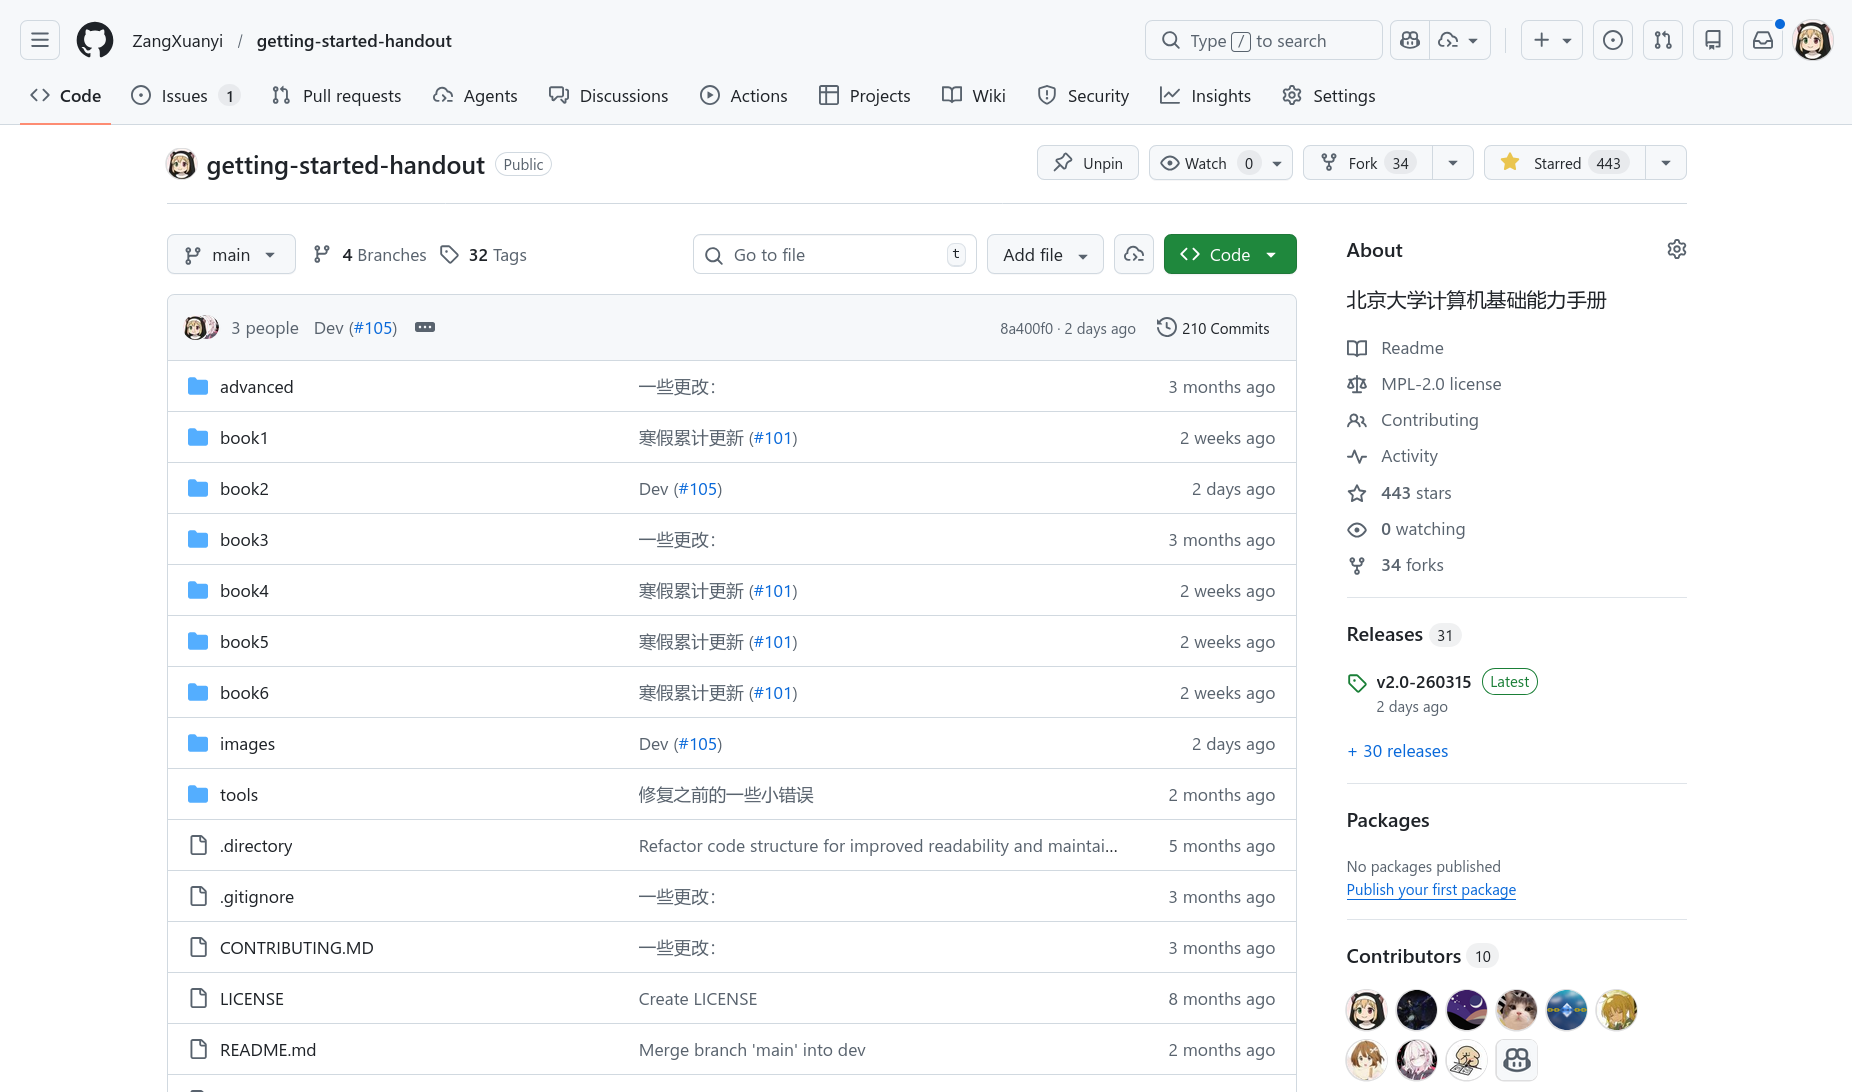
\includegraphics[width=0.8\textwidth]{gh.png}
    \end{figure}

\end{frame}

\begin{frame}
    \frametitle{PR、Issue}

    PR（Pull Request）实际上就是带审查的merge。提出PR者一般会在PR里写一些说明，告诉审查者这个PR的目的是什么，改了哪些内容等等。审查者可以在PR里进行评论，提出修改意见，甚至直接修改代码（如果有权限的话）。当审查者认为PR已经准备好被合并了，就可以进行merge了。

    \hspace{2em}

    Issue用于跟踪和管理项目中的任务、功能请求、错误报告等。它是一个非常重要的工具，可以帮助团队成员更好地协作和沟通。

\end{frame}

\begin{frame}
    \frametitle{关于Vibe Coding}

    上课的时候，刘老师说，Vibe Coding 是一个非常好的工具，可以借助LLM的能力来帮助我们更高效地编写代码。它可以提供智能的代码补全、错误检查、代码重构等功能，极大地提升了我们的编码效率和代码质量。

    \textbf{但是，我个人非常建议同学们不要过于依赖Vibe Coding}，甚至远离Vibe Coding。

    我个人认为，Vibe的前提必须是：
    \begin{itemize}
        \item 你自己会写，实在是懒得写（即完成重复工作）；
        \item 你有着足够的能力，能够分辨代码的好坏，能够对Vibe生成的代码进行修改和优化。
    \end{itemize}


\end{frame}

\begin{frame}
    \frametitle{一点题外话}

    如果上述条件都不满足，那我非常建议你\textbf{先查阅资料、询问LLM，确保自己能力足够、真会了之后，再去Vibe提升效率}。

    \textbf{不要变成拿着枪的猴子。}新手更是如此：我们都知道大学生经常按计算器，但哪里有还没学会算术的小学生按计算器的？

    \textbf{\alert{做自己代码的第一责任人。}}

    \hspace{2em}

    \small

    那日，有聪明的童女拿着灯，却不预备油。

    她们对愚拙的说：“请分点油给我们。”

    愚拙的却回答说：“恐怕不够你我用的，不如你们自己到卖油的那里去买。”

    这话是真实的。

    因为各人要喝自己的杯，各人要行自己的路。

    —— 仿自《圣经》
\end{frame}

\begin{frame}
    \frametitle{不要这样}

    \begin{figure}
        \centering
        
\includegraphics[width=0.4\textwidth]{shit.jpg}
    \end{figure}

\end{frame}

\begin{frame}
    \frametitle{常见开源协议}
    开源协议一般管的是代码的使用、修改、分发等方面的权利和义务。不同的开源协议有不同的规定，主要可以分为左、中、右三类：
    \begin{description}
            \color{red}
        \item[AGPL] 联网使用即开源整个项目
        \item[GPL] 分发即开源整个项目
        \item[LGPL] 直接修改的整个库需开源
        \item[MPL] 直接修改的单个文件本身需开源
            \color{black}
        \item[Apache] 有专利权、有版权
        \item[BSD、MIT] 未提及专利权、有版权
        \item[Unlicenced] 放弃所有权利
            \color{blue}
        \item[商业许可证] 本质上是商业合同
    \end{description}
    张三直接挪用李四写的GPL的演示文稿、MPL的《手册》却没有署名李四，李四可以起诉张三侵权。
\end{frame}

\begin{frame}
    \frametitle{常见知识产权保护协议}

    与上述开源协议不同，这些协议保护的是文字、图像创作者的权利，它们通常用于保护作品不被未经授权的使用、复制、修改等。一般BY：by，署名；SA：share alike，相同方式共享；ND：no derivatives，禁止演绎（禁止修改）；NC：non-commercial，非商业性使用。

    \begin{description}
        \item[CC BY] 署名
        \item[CC BY-SA] 署名-相同方式共享
        \item[CC BY-ND] 署名-禁止演绎
        \item[CC BY-NC] 署名-非商业性使用
        \item[CC BY-NC-SA] 署名-非商业性使用-相同方式共享
        \item[CC BY-NC-ND] 署名-非商业性使用-禁止演绎
        \item[CC0] 放弃所有权利
    \end{description}

\end{frame}

\begin{frame}
    \frametitle{常见开源社区}
    和开源协议一样，也分左中右。

    左派（自由软件派）：Mozilla、KDE、GNOME、GNU，大多采用GPL、LGPL协议。

    中间派（开源实用派）：Linux各大发行版、LLVM、商业公司运营的开源社区（如Microsoft、Google等）。

    右派（生态封闭派）：Apple的Swift（开源代码，但生态封闭），Oracle的MySQL（开源代码，双授权）等。


\end{frame}

\end{document}